\section{Appendix}

\setcounter{table}{0}
\renewcommand{\thetable}{A\arabic{table}}
\setcounter{figure}{0}
\renewcommand{\thefigure}{A\arabic{figure}}


\subsection{Stan Code}
This section contains the \texttt{Stan} model code for both the exponential and Weibull survival model. Additional \texttt{R}-code is available on \href{https://github.com/pitrieger/BayesianStats_FinalProject}{GitHub}.

\begin{lstlisting}[language=Stan, caption = {Exponential Survival Model}, captionpos = t, label = {code:stan_exp}]
data {
    int<lower=0> n_event; // # uncensored obs                                     
    int<lower=0> n_censor; // # censored obs                                    
    int<lower=0> p; // # covariates excluding intercept                                        
    matrix[n_event,p] X_event; // uncensored obs design matrix                           
    matrix[n_censor,p] X_censor; // censored  -----"---------- 
    matrix[3,p] X_pred; // for posterior predictive distribution
    vector<lower=0>[n_event] T_event; // uncensored survival times                         
    vector<lower=0>[n_censor] T_censor; // lower bound of censored survival times = censor time                  
}
parameters {
    real alpha;
    vector[p] beta;                                     
}
transformed parameters{
    vector[n_event] lambda_event = exp(alpha + X_event * beta);
    vector[n_censor] lambda_censor = exp(alpha + X_censor * beta);
}
model {
    alpha ~ normal(0, 100);
    beta ~ normal(0, 5);
    target += exponential_lpdf(T_event | lambda_event); 
    target += exponential_lccdf(T_censor | lambda_censor);  
}
generated quantities {
  vector[n_event + n_censor] T_hat;
  vector[3] T_pred;
  for(i in 1:n_event){
    T_hat[i] = exponential_rng(lambda_event[i]);
  }
  for(i in 1:n_censor){
    T_hat[i + n_event] = exponential_rng(lambda_censor[i]);
  }
  for(i in 1:3){
    T_pred[i] = exponential_rng(exp(alpha + X_pred * beta)[i]);
  }
  
}
\end{lstlisting}

\clearpage

\begin{lstlisting}[language=Stan, caption = {Weibull Survival Model}, captionpos = t, label = {code:stan_weib}]
data {
    int<lower=0> n_event; // # uncensored obs                                     
    int<lower=0> n_censor; // # censored obs                                    
    int<lower=0> p; // # covariates excluding intercept                                        
    matrix[n_event,p] X_event; // uncensored obs design matrix                           
    matrix[n_censor,p] X_censor; // censored  -----"----------
    matrix[3,p] X_pred; // for posterior predictive distribution
    vector<lower=0>[n_event] T_event; // uncensored survival times                         
    vector<lower=0>[n_censor] T_censor; // lower bound of censored survival times = censor time                  
}
parameters {
  real mu;
  vector[p] beta;
  real<lower = 0> alpha;
}
transformed parameters {
  vector[n_event] sigma_event = exp(- (mu + X_event * beta)/ alpha);
  vector[n_censor] sigma_censor = exp(- (mu + X_censor * beta)/ alpha);
}

model {
  mu ~ normal(0, 100);
  beta ~ normal(0, 5);
  alpha ~ cauchy(0, 2.5);
  target += weibull_lpdf(T_event | alpha, sigma_event);
  target += weibull_lccdf(T_censor | alpha, sigma_censor);
}
generated quantities {
  vector[n_event + n_censor] T_hat;
  vector[3] T_pred;
  for(i in 1:n_event){
    T_hat[i] = weibull_rng(alpha, sigma_event[i]);
  }
  for(i in 1:n_censor){
    T_hat[i + n_event] = weibull_rng(alpha, sigma_censor[i]);
  }
  for(i in 1:3){
    T_pred[i] = weibull_rng(alpha, exp(- (mu + X_pred * beta)/ alpha)[i]); 
  }
}
\end{lstlisting}


\subsection{Weibull Survival Model}
This section contains the coefficient plot for the Weibull model, which was excluded from the main section because it does not differ substantially from the coefficient plot for the exponential model, shown in Figure \ref{fig:exp_coefplot}. 

\begin{figure}
    \centering
    \minp{\caption{Posterior densities of the coefficients in the Weibull survival model.} \label{fig:weib_coefplot}}
    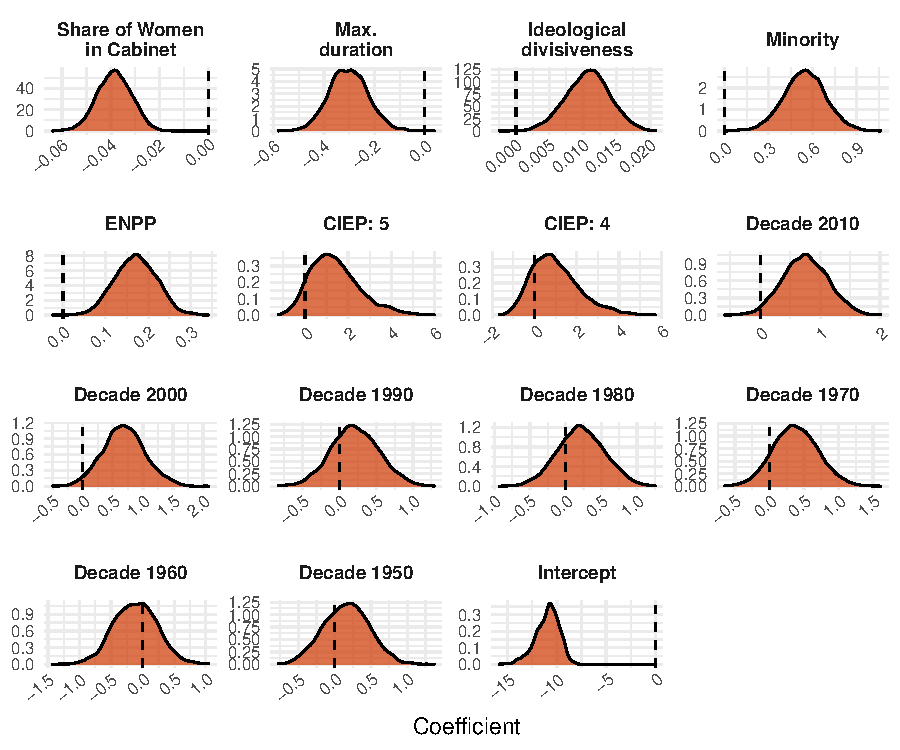
\includegraphics[width = 0.8\textwidth]{figures/fig1_weib_coefplot.pdf}
\end{figure}


\subsection{Zero-Inflated Poisson Regression}
Since the main interest of \textcite{KK20} and this paper does not lie in the concrete survival times, but rather on the association between government stability and the share of female ministers in the cabinet, the problem can also be approached differently, i.e. outside the survival modelling framework. It is generally known when the next regular elections will be held. At the time of government formation, we can thus already tell what the maximum number of possible days in office for that government will be. In fact, this is used as one of the covariates in the survival models in the paper. Denoting this maximum as $m_i$, we can compute the number of days that the government fell short of reaching that maximum as 

\begin{equation*}
    \widetilde{Y}_i = m_i - Y_i.
\end{equation*}

We thus have a count variable $\widetilde{Y}_i$ that can be modelled as a zero-inflated Poisson random variable. The likelihood of this model is therefore given by 

\begin{equation*}
    \mathcal{L}_i(\theta) = \begin{cases}
    \pi_i + (1-\pi_i) e^{-\lambda_i} \lambda_i^{0} & \text{, $\tilde{y}_i = 0$} \\
    (1-\pi_i) \frac{e^{-\lambda_i} \lambda_i^{y_i}}{\tilde{y}_i!} & \text{, otherwise}
    \end{cases}
\end{equation*}

where $\bm\theta = (\bm\pi, \bm\lambda)$ can be defined via logistic and log link functions, respectively, such that 

\begin{align*}
    \bm\pi &= (1 + \exp(-(\beta_0 + \bm{X} \bm\beta)))^{-1} \\
    \bm\lambda &= \exp(\gamma_0 + \bm{Z} \bm\gamma). 
\end{align*}

\texttt{Stan} and \texttt{R}-code for this model are included in the \href{https://github.com/pitrieger/BayesianStats_FinalProject}{GitHub repository of this paper}. However, the parameters of the zero-inflation component fail to converge properly when using the full set of covariates for both $\bm{X}$ and $\bm{Z}$. When using certain subsets $\bm{Z}' \subset \bm{Z}$ and the full set of covariates $\bm{X}$, the model yields results that are equivalent to the survival models discussed in this paper. 
